\section{Auswertung}
\label{sec:Auswertung}
\subsection{Ablenkung von Elektronen durch das Magnetfeld}
In Tabelle \ref{tab:DIS} sind die Stromstärken $I_\text{S}$ zu den Entsprechenden Auslenkungen $D$ aufgetragen.
\begin{table}
  \centering
  \begin{tabular}{c| c c c c c }
    \toprule
    $D / \frac{Zoll}{4}$ & $U_\text{B}$ = 250 V & $U_\text{B}$ = 300 V & $U_\text{B}$ = 350 V & $U_\text{B}$ = 400 V & $U_\text{B}$ = 450 V \\
    \midrule
    1 &	0	&0	&0	&0	&0	\\
    2 &	0.27	&0.34	&0.37	&0.42	&0.41	\\
    3 &	0.63	&0.70	&0.74	&0.83	&0.85	\\
    4 &	0.95	&1.05	&1.15	&1.25	&1.30	\\
    5 &	1.27	&1.40	&1.55	&1.61	&1.73	\\
    6 &	1.57	&1.76	&1.91	&2.01	&2.15	\\
    7 &	1.92	&2.11 	&2.27	&2.47	&2.59	\\
    8 &	2.23	&2.45	&2.67	&2.91	&3.02	\\
    9 &	2.53	&2.81	&3.02	&/	&/	\\
    \bottomrule
  \end{tabular}
  \caption{Auslenkung der Elektronen in Abhägigkeit des Spulenstroms bei unterschiedlichen Beschleunigungsspannungen}
  \label{tab:DIS}
\end{table}
Anhand derer lassen sich durch verwendung von Gleichung \eqref{eqn:BH} die magnetischen Feldstärken errechnen. Diese werden in Diagramm \ref{fig:bfeld} gegen $D/(L^2+D^2)$ aufgetragen sowie ein linearer Fit durch die Messpunkte gelegt.
\begin{figure}
  \centering
  \includegraphics[height=7cm]{B-Feld.pdf}
  \caption{Diagramm zur Bestimmung der spezifischen Ladung}
  \label{fig:bfeld}
\end{figure}
Aus den Steigungen $a$ der Fitts lassen sich durch Umformung der Gleichung \eqref{eqn:e0m} zu,
\begin{equation}
  \frac{e_0}{m_0} = \left( a \cdot \sqrt{8 U_\text{B}} )^2 \right)
  \label{eqn:e0m0}
\end{equation}
die spezifische Ladung der Elektronen berechnen. Diese sind mit den zugehörigen Beschleunigungspannungen und ihrer relativen Abweichung von ihrem Literaturwert (\cite{spez}) in Tabelle \ref{tab:e0m0} aufgetragen.
\begin{table}
  \centering
  \begin{tabular}{c| c c}
    \toprule
    $U_\text{B}$  & $e_0/m_0$ praktisch & $\Delta e_0/m_0$ \\
    \midrule
    	250	& (\num{1.77 +- 0.05}) & 1 \% \\
	300	& (\num{1.76 +- 0.05}) & 1 \% \\
	350	& (\num{1.76 +- 0.04}) & 1 \% \\
	400	& (\num{1.78 +- 0.07}) & 1 \% \\
	450	& (\num{1.80 +- 0.04}) & 2 \% \\
    \bottomrule
  \end{tabular}
  \caption{spezifische Ladung und Abweichung vom Literaturwert}
  \label{tab:e0m0}
\end{table}
\subsection{Intensität des Erdmagnetfeld}
Für den Versuch wird ein Inktlisationswinkel von
\begin{equation}
  \Phi_\text{Inc} = (\num{66 +-3})°
  \label{eqn:Inc}
\end{equation}
gemessen. Der Strom $I_\text{K}$ um das Magnetfeld der Erde mittels Helmholzspulen zu kompensieren beträgt
\begin{equation}
  I_\text{K} = 0.27 \, \text{A} \ .
  \label{IK}
\end{equation}
Mit Formel \eqref{eqn:BH} ergibt sich für den Strom $I_\text{K}$ ein magnetisches Feld von
\begin{equation}
  B_\text{Helm} = 1.72 \cdot 10^{-5} \, \text{T} \ .
  \label{eqn:Binc}
\end{equation}
Nach Bereinigung des magnetischen Feldes von dem Inklisationswinkel ergibt sich eine Totalintesistät von
\begin{equation}
  B_\text{Erd} = 4.34 \cdot 10^{-5} \, \text{T} \ .
  \label{eqn:Berd}
\end{equation}
\subsection{Empfindlichkeit der Braunschen Röhre}
In einem linearen Diagramm werden die Ablenkspannungen $U_\text{d}$ aus Tabelle \ref{tab:DIS} gegen die Verschiebung $D$ des Leuchtflecks aufgetragen.
\begin{table}
  \centering
  \begin{tabular}{c| c c c c c }
    \toprule
    $D / \frac{Zoll}{4}$ & $U_\text{B}$ = 180 V & $U_\text{B}$ = 230 V & $U_\text{B}$ = 260 V & $U_\text{B}$ = 300 V & $U_\text{B}$ = 350 V \\
    \midrule
    1 &	-20.02	&-25.21	&-28.00	&-32.19	&-28.00	\\
    2 &	-16.12	&-20.24	&-22.99	&-27.04	&-22.99	\\
    3 &	-12.64	&-16.07	&-18.05	&-21.16	&-18.05	\\
    4 &	-8.88	&-12.18	&-12.65	&-15.28	&-12.65	\\
    5 &	-5.10	&-7.59	&-7.51	&-9.58	&-7.51	\\
    6 &	-1.37	&-2.69	&-2.64	&-4.02	&-2.64	\\
    7 &	2.62	&2.04	&2.73	&2.17	&2.73	\\
    8 &	6.53	&6.79	&8.34	&7.97	&8.34	\\
    9 &	10.44	&11.60	&13.57	&14.40	&13.57	\\
    \bottomrule
  \end{tabular}
  \caption{Auslenkung der Elektronen in Abhängigkeit der Ablenkspannung bei unterschiedlichen Beschleunigungsspannungen}
  \label{tab:DIS}
\end{table}
\begin{figure}
  \centering
  \includegraphics[height=8cm]{E-Feld.pdf}
  \caption{Empfindlichkeit der Braunschen Röhre}
  \label{fig:empf}
\end{figure}
Es wird ein Fit durch die einzelnen Messpunkte gelegt anhand derer die Empfindlichkeit der Braunschen Röhre bestimmt wird. Diese wird in einem weiterem Diagramm gegen den Kehrwert der Beschleunigungsspannung aufgetragen.
\begin{figure}
  \centering
  \includegraphics[height=8cm]{E-Feld2.pdf}
  \caption{Bestimmtung der Kenngröße}
  \label{fig:K}
\end{figure}
Anhand der Steigung des weiteren Fits lässt sich die Kenngröße
\begin{equation}
  K_\text{theo} = \frac{p L}{2 d} = \frac{0.019 \, \text{m} \cdot 0.143 \, \text{m}}{2 \cdot 0.006 \, \text{m}} = 0.226 \, \frac{1}{\text{m}}
  \label{eqn:Ktheo}
\end{equation}
des Systems bestimmen. Der Fit liefert eine Kenngröße von
\begin{equation}
  K_\text{Messung} = (\num{0.27 +- 0.01}) \, \frac{1}{\text{m}} \ .
  \label{Kmess}
\end{equation}
\subsection{Kathodenstrahl-Oszillograph}
Die gemessene Frequenzverhältnisse sind in Tabelle \ref{tab:sync} aufgeführt.
\begin{table}
  \centering
  \begin{tabular}{c c c}
    \toprule
    Frequenzverhältniss & $\nu_\text{Messung}$ & $\nu_\text{Theoretisch}$ \\
    \midrule
    1:2	& 159.96& 160.00\\
    1:1	& 79.75 & 80.00	\\
    2:1	& 39.87 & 40.00	\\
    3:1	& 26.65 & 26.67	\\
    \bottomrule
  \end{tabular}
  \caption{Synchronisationsfrequenzen}
  \label{tab:sync}
\end{table}
Ein Bild einer stehenden Welle ist in Abbildung \ref{fig:pic} zu sehen.
\begin{figure}
  \centering
  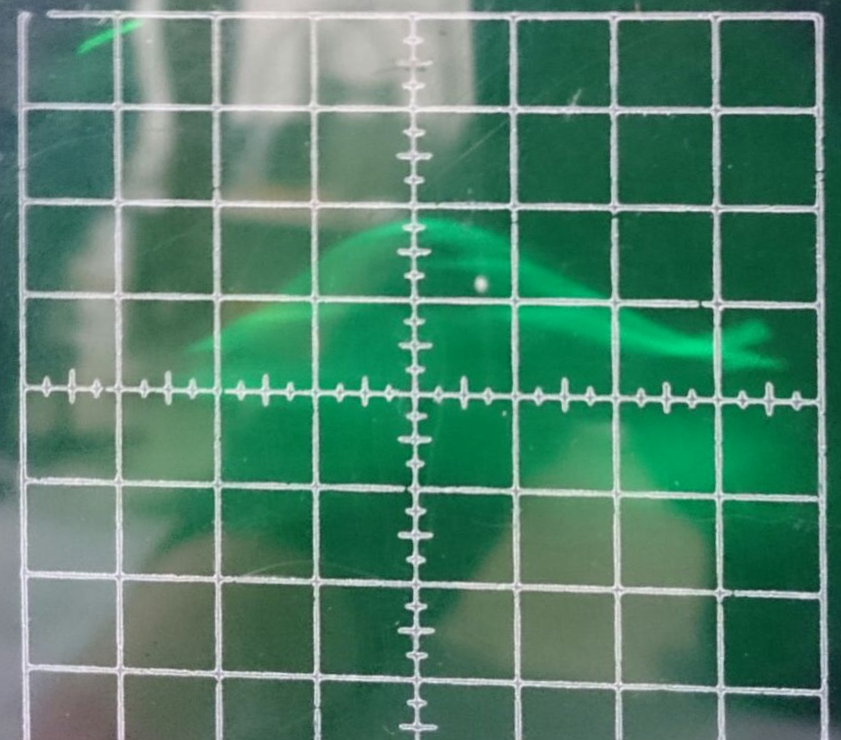
\includegraphics[height=7cm]{picture/sinus.png}
  \caption{Stehende Sinuswelle}
  \label{fig:pic}
\end{figure}
Aus Mittelung der mit dem Frequenzverhältnis multiplizierten gemessenen Frequenzen ergibt sich eine mittlere Frequenz von
\begin{equation}
  \overline{\nu_\text{Messung}} = \num{79.81 +- 0.05} \text{Hz}
  \label{eqn:numess}
\end{equation}
Desweiteren soll der Schwellwert der Spannung $U_\text{B}$ werden. Da die Empfindlichkeit der Röhre bereits bekannt ist, ergibt dieser sich durch Umformen der Gleichung \eqref{eqn:DUd} nach $U_d$ zu
\begin{equation}
  U_\text{d} = \frac{D 2 d U_\text{B}}{p L} \ .
  \label{eqn:dfs}
\end{equation}
Für die Beschleunigungsspannung von 260 V Ergibt sich für die verschiedenen Verschiebungen $D$ auf dem Schirm die in der Tabelle \ref{tab:scheitel} aufgeführten Scheitelwerte.
\begin{table}
  \centering
  \begin{tabular}{c c c}
    \toprule
	Frequenzverhältniss & D / mm & $U_\text{d}$ / V \\
    \midrule
	1:2	& 6.3 & 5.2 	\\
	1:1	& 6.3 & 5.2	\\
	2:1	& 5.7 & 4.7	\\
	3:1	& 5.7 & 4.7	\\
    \bottomrule
  \end{tabular}
  \caption{Verschiebung und Scheitelwert der Spannung}
  \label{tab:scheitel}
\end{table}
